% BSG-IDE User Manual
% Please create a file named 'BSG-IDE_user_manual.tex' with this content

\documentclass[11pt,a4paper]{article}

\usepackage[utf8]{inputenc}
\usepackage[T1]{fontenc}
\usepackage{lmodern}
\usepackage[margin=2.5cm]{geometry}
\usepackage{tikz}
\usepackage{listings}
\usepackage{xcolor}
\usepackage{hyperref}
\usepackage{graphicx}
\usepackage{float}
\usepackage{enumitem}
\usepackage{tcolorbox}
\usepackage{fancyhdr}
\usepackage{chngcntr}
\usepackage{amssymb} % to add checkmark
\usepackage{multicol}
\usepackage{makeidx}
% Reset figure numbers for each section
\counterwithin{figure}{section}

% TikZ libraries
\usetikzlibrary{shapes,arrows,positioning,backgrounds,fit,shadows,arrows.meta}

% Colors
\definecolor{codebg}{RGB}{240,240,240}
\definecolor{codegreen}{RGB}{28,172,120}
\definecolor{codelightblue}{RGB}{32,162,242}
\definecolor{codedarkblue}{RGB}{18,39,135}

\hypersetup{
    colorlinks=true,
    linkcolor=blue,
    filecolor=magenta,
    urlcolor=cyan,
}
% Listing settings
\lstset{
    language=Python,
    backgroundcolor=\color{codebg},
    basicstyle=\small\ttfamily,
    keywordstyle=\color{codedarkblue}\bfseries,
    stringstyle=\color{codegreen},
    commentstyle=\color{gray},
    numbers=left,
    numberstyle=\tiny,
    frame=single,
    breaklines=true,
    showstringspaces=false
}

% Page style
\pagestyle{fancy}
\fancyhf{}
\fancyhead[L]{BSG-IDE User Manual}
\fancyhead[R]{\thepage}
\renewcommand{\headrulewidth}{0.4pt}

\begin{document}

\begin{titlepage}
    \centering
    \vspace*{3cm}
    {\Huge \textbf{BSG-IDE User Manual}\par}
    \vspace{2cm}
    {\Large Beamer Slide Generator Integrated Development Environment\par}
    \vspace{3cm}
    {\large{Ninan Sajeeth Philip}\par}
    {\large Version 1.0.0\par}
    \vspace{2cm}
    {\large \today\par}
    \vspace{3cm}
    {\large Artificial Intelligence Research and Intelligent Systems (airis4D)\par}
     {\large where we Dream, Design, Develop and Deploy Future Technologies\par}
\end{titlepage}

\tableofcontents
\newpage

\section{Introduction}

BSG-IDE (Beamer Slide Generator Integrated Development Environment) is a comprehensive tool designed to streamline the creation of Beamer presentations. It combines a user-friendly interface with powerful features for managing slides, media content, and presentation notes.

\begin{figure}[H]
\centering
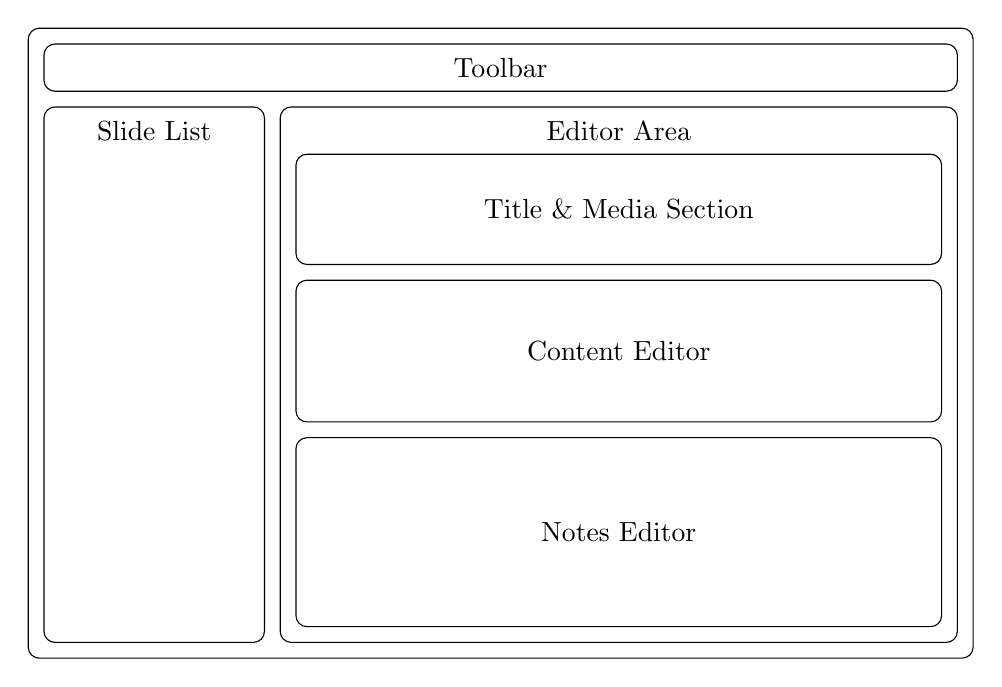
\begin{tikzpicture}
    \begin{scope}
        % Main window
        \draw [rounded corners] (0,0) rectangle (12,-8);

        % Toolbar
        \draw [rounded corners] (0.2,-0.2) rectangle (11.8,-0.8);
        \node at (6,-0.5) {Toolbar};

        % Sidebar
        \draw [rounded corners] (0.2,-1) rectangle (3,-7.8);
        \node at (1.6,-1.3) {Slide List};

        % Main editor
        \draw [rounded corners] (3.2,-1) rectangle (11.8,-7.8);
        \node at (7.5,-1.3) {Editor Area};

        % Components in main editor
        \draw [rounded corners] (3.4,-1.6) rectangle (11.6,-3);
        \node at (7.5,-2.3) {Title \& Media Section};

        \draw [rounded corners] (3.4,-3.2) rectangle (11.6,-5);
        \node at (7.5,-4.1) {Content Editor};

        \draw [rounded corners] (3.4,-5.2) rectangle (11.6,-7.6);
        \node at (7.5,-6.4) {Notes Editor};
    \end{scope}
\end{tikzpicture}
\caption{BSG-IDE Main Interface Layout}
\end{figure}

\section{Installation}

\subsection{System Requirements}
\begin{itemize}
    \item Python 3.8 or higher
    \item LaTeX distribution (TeXLive or MiKTeX)
    \item Internet connection for initial setup
    \item Minimum 4GB RAM recommended
    \item 1GB free disk space
\end{itemize}

\subsection{Installation Process}
The installation process is automated and handles all dependencies:

\begin{lstlisting}[caption=Installation Command]
python3 BSG-IDE.py --fix
\end{lstlisting}

This command:
\begin{itemize}
    \item Creates a virtual Python environment
    \item Installs required packages
    \item Sets up desktop integration
    \item Creates necessary directories
\end{itemize}

\begin{tcolorbox}[title=Note]
If you encounter any installation issues, you can rerun the installation with the --fix flag to repair the installation.
\end{tcolorbox}

\section{User Interface}

\subsection{Main Components}

\begin{enumerate}
    \item \textbf{Toolbar} - Contains primary actions:
        \begin{itemize}
            \item New Presentation
            \item Open
            \item Save
            \item Convert to TeX
            \item Generate PDF
            \item Preview
        \end{itemize}

    \item \textbf{Slide List} - Shows all slides with:
        \begin{itemize}
            \item Slide titles
            \item Current slide indicator
            \item Drag-and-drop reordering
        \end{itemize}

    \item \textbf{Editor Area} - Three main sections:
        \begin{itemize}
            \item Title and media section
            \item Content editor
            \item Notes editor
        \end{itemize}
\end{enumerate}

\subsection{Editor Features}

\begin{figure}[H]
\centering
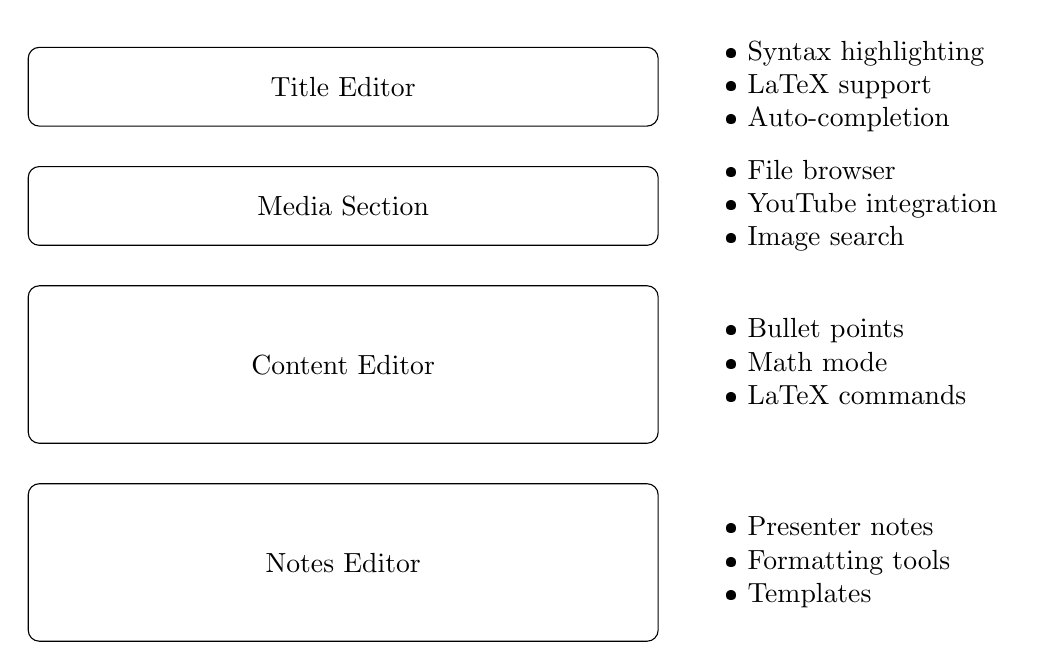
\begin{tikzpicture}
    \begin{scope}[node distance=2cm]
        % Editor components
        \node[rectangle, draw, rounded corners, minimum width=8cm, minimum height=1cm] (title) {Title Editor};
        \node[rectangle, draw, rounded corners, minimum width=8cm, minimum height=1cm, below=0.5cm of title] (media) {Media Section};
        \node[rectangle, draw, rounded corners, minimum width=8cm, minimum height=2cm, below=0.5cm of media] (content) {Content Editor};
        \node[rectangle, draw, rounded corners, minimum width=8cm, minimum height=2cm, below=0.5cm of content] (notes) {Notes Editor};

        % Features
        \node[right=0.5cm of title] (title-features) {\begin{tabular}{l}
            • Syntax highlighting\\
            • LaTeX support\\
            • Auto-completion
        \end{tabular}};

        \node[right=0.5cm of media] (media-features) {\begin{tabular}{l}
            • File browser\\
            • YouTube integration\\
            • Image search
        \end{tabular}};

        \node[right=0.5cm of content] (content-features) {\begin{tabular}{l}
            • Bullet points\\
            • Math mode\\
            • LaTeX commands
        \end{tabular}};

        \node[right=0.5cm of notes] (notes-features) {\begin{tabular}{l}
            • Presenter notes\\
            • Formatting tools\\
            • Templates
        \end{tabular}};
    \end{scope}
\end{tikzpicture}
\caption{Editor Components and Features}
\end{figure}

\section{Working with Media}

\subsection{Supported Media Types}
\begin{itemize}
    \item \textbf{Images:} PNG, JPG, JPEG, PDF
    \item \textbf{Videos:} MP4, AVI, MOV, WebM
    \item \textbf{Web Content:} YouTube videos, URLs
    \item \textbf{Vector Graphics:} SVG, EPS
\end{itemize}

\subsection{Media Browser}
\begin{figure}[H]
\centering
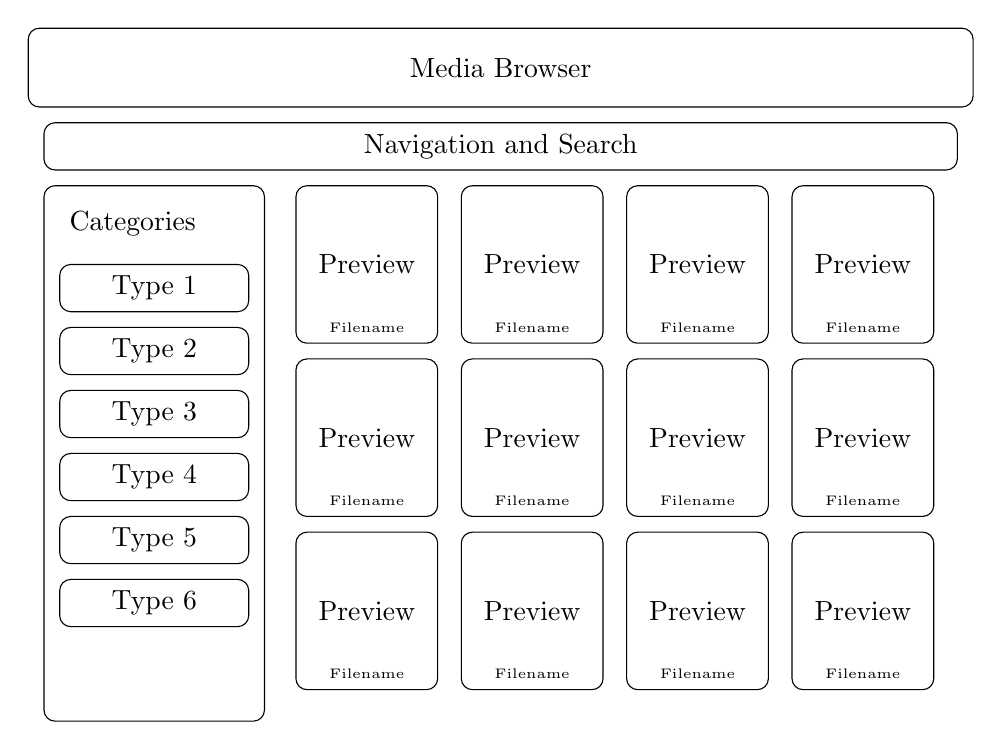
\begin{tikzpicture}
    \begin{scope}
        % Media browser window
        \draw [rounded corners] (0,0) rectangle (12,1);
        \node at (6,0.5) {Media Browser};

        % Navigation bar
        \draw [rounded corners] (0.2,-0.2) rectangle (11.8,-0.8);
        \node at (6,-0.5) {Navigation and Search};

        % Left panel - Categories
        \draw [rounded corners] (0.2,-1) rectangle (3,-7.8);
        \begin{scope}[node distance=0.5cm]
            \node[anchor=north west] at (0.4,-1.2) {Categories};
            \foreach \y in {1,...,6} {
                \draw [rounded corners] (0.4,-1.2-\y*0.8) rectangle (2.8,-1.8-\y*0.8);
                \node at (1.6,-1.5-\y*0.8) {Type \y};
            }
        \end{scope}

        % Thumbnail grid
        \begin{scope}[shift={(3.2,-3)}]
            \foreach \x in {0,...,3} {
                \foreach \y in {0,...,2} {
                    \draw [rounded corners] (\x*2.1+0.2,-\y*2.2) rectangle (\x*2.1+2,-\y*2.2+2);
                    \node at (\x*2.1+1.1,-\y*2.2+1) {Preview};
                    \node[font=\tiny] at (\x*2.1+1.1,-\y*2.2+0.2) {Filename};
                }
            }
        \end{scope}
    \end{scope}
\end{tikzpicture}
\caption{Media Browser Interface}
\end{figure}

\subsection{Media Management Features}
The integrated media browser provides:
\begin{itemize}
    \item Real-time thumbnail generation
    \item Automatic file categorization
    \item Search and filter capabilities
    \item Drag-and-drop support
    \item Quick preview functionality
    \item File metadata display
\end{itemize}

\section{Presentation Notes}

\subsection{Notes Functionality}
\begin{figure}[H]
\centering
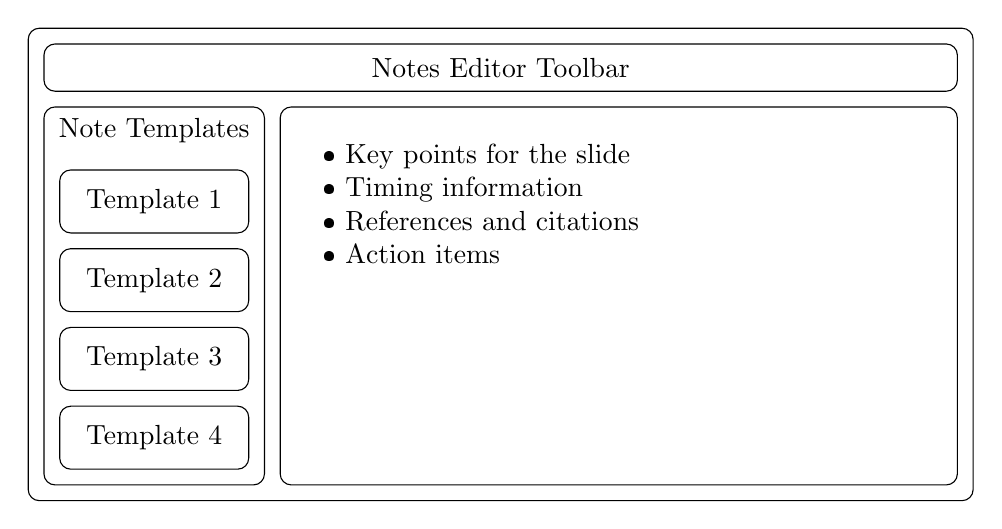
\begin{tikzpicture}
    \begin{scope}
        % Notes editor interface
        \draw [rounded corners] (0,0) rectangle (12,-6);

        % Toolbar
        \draw [rounded corners] (0.2,-0.2) rectangle (11.8,-0.8);
        \node at (6,-0.5) {Notes Editor Toolbar};

        % Left panel - Templates
        \draw [rounded corners] (0.2,-1) rectangle (3,-5.8);
        \node at (1.6,-1.3) {Note Templates};
        \foreach \y in {0,...,3} {
            \draw [rounded corners] (0.4,-1.8-\y*1) rectangle (2.8,-2.6-\y*1);
            \node at (1.6,-2.2-\y*1) {Template \number\numexpr\y+1\relax};
        }

        % Main notes area
        \draw [rounded corners] (3.2,-1) rectangle (11.8,-5.8);
        \node[anchor=north west] at (3.4,-1.3) {\begin{tabular}{l}
            • Key points for the slide\\
            • Timing information\\
            • References and citations\\
            • Action items\\
            \end{tabular}};
    \end{scope}
\end{tikzpicture}
\caption{Notes Editor Interface}
\end{figure}

\subsection{Note Types and Templates}
The IDE supports various note templates:
\begin{itemize}
    \item \textbf{Key Points} - Main talking points and highlights
    \item \textbf{Time Markers} - Presentation timing guidelines
    \item \textbf{Action Items} - Follow-up tasks and reminders
    \item \textbf{References} - Citations and source materials
    \item \textbf{Technical Notes} - Detailed technical information
\end{itemize}

\section{Syntax Highlighting}

\subsection{Code Highlighting Features}
\begin{figure}[H]
\centering
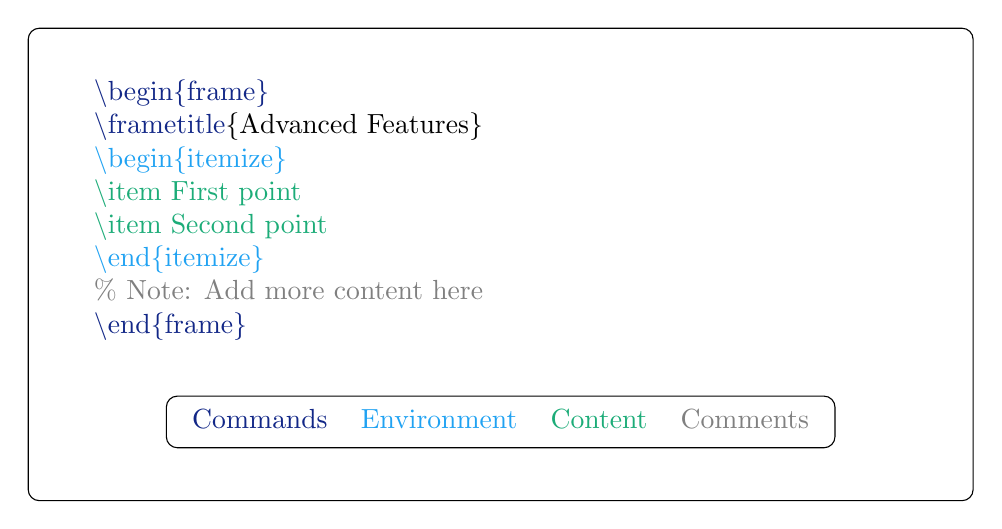
\begin{tikzpicture}
    \begin{scope}
        % Code editor window
        \node[rectangle, draw, rounded corners, minimum width=12cm, minimum height=6cm] (editor) at (0,0) {};

        % Code sample with syntax highlighting
        \node[anchor=north west] at (-5.5,2.5) {
            \begin{tabular}{l}
                \textcolor{codedarkblue}{\textbackslash begin\{frame\}} \\
                \textcolor{codedarkblue}{\textbackslash frametitle}\{Advanced Features\} \\
                \textcolor{codelightblue}{\textbackslash begin\{itemize\}} \\
                \textcolor{codegreen}{\textbackslash item First point} \\
                \textcolor{codegreen}{\textbackslash item Second point} \\
                \textcolor{codelightblue}{\textbackslash end\{itemize\}} \\
                \textcolor{gray}{\% Note: Add more content here} \\
                \textcolor{codedarkblue}{\textbackslash end\{frame\}}
            \end{tabular}
        };

        % Legend
        \node[rectangle, draw, rounded corners] at (0,-2) {
            \begin{tabular}{l l l l}
                \textcolor{codedarkblue}{Commands} &
                \textcolor{codelightblue}{Environment} &
                \textcolor{codegreen}{Content} &
                \textcolor{gray}{Comments}
            \end{tabular}
        };
    \end{scope}
\end{tikzpicture}
\caption{Syntax Highlighting Example}
\end{figure}

\section{Advanced Features}

\subsection{Terminal Integration}
\begin{figure}[H]
\centering
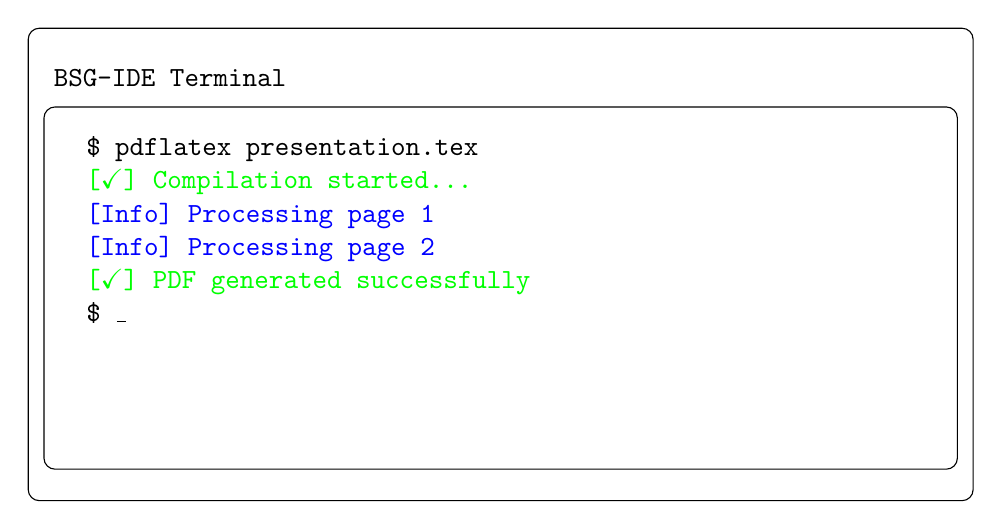
\begin{tikzpicture}
    \begin{scope}
        % Terminal window
        \draw [rounded corners] (0,0) rectangle (12,-6);
        \node[anchor=north west] at (0.2,-0.4) {\texttt{BSG-IDE Terminal}};

        % Command line interface
        \begin{scope}[yshift=-1cm]
            \draw [rounded corners] (0.2,0) rectangle (11.8,-4.6);
            \node[anchor=north west, font=\ttfamily] at (0.4,-0.2) {
                \begin{tabular}{l}
                    \$ pdflatex presentation.tex\\
                    \textcolor{green}{[\checkmark] Compilation started...}\\
                    \textcolor{blue}{[Info] Processing page 1}\\
                    \textcolor{blue}{[Info] Processing page 2}\\
                    \textcolor{green}{[\checkmark] PDF generated successfully}\\
                    \$ \_
                \end{tabular}
            };
        \end{scope}
    \end{scope}
\end{tikzpicture}
\caption{Integrated Terminal Interface}
\end{figure}

\subsection{Real-time PDF Preview}
\begin{figure}[H]
\centering
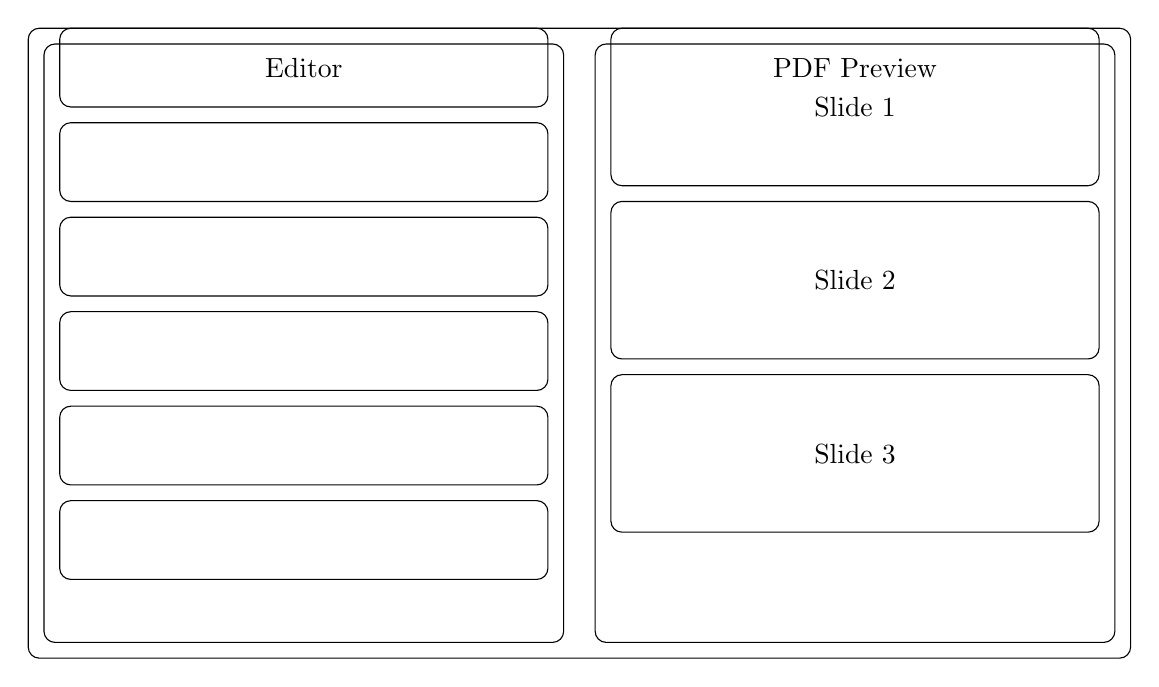
\begin{tikzpicture}
    \begin{scope}
        % Main window
        \draw [rounded corners] (0,0) rectangle (14,-8);

        % Editor pane
        \draw [rounded corners] (0.2,-0.2) rectangle (6.8,-7.8);
        \node at (3.5,-0.5) {Editor};

        % Preview pane
        \draw [rounded corners] (7.2,-0.2) rectangle (13.8,-7.8);
        \node at (10.5,-0.5) {PDF Preview};

        % Sample content
        \begin{scope}[shift={(0.4,-1)}]
            \foreach \y in {0,...,5} {
                \draw [rounded corners] (0,-\y*1.2) rectangle (6.2,-\y*1.2+1);
            }
        \end{scope}

        % Sample PDF pages
        \begin{scope}[shift={(7.4,-2)}]
            \foreach \y in {0,...,2} {
                \draw [rounded corners] (0,-\y*2.2) rectangle (6.2,-\y*2.2+2);
                \node at (3.1,-\y*2.2+1) {Slide \number\numexpr\y+1\relax};
            }
        \end{scope}
    \end{scope}
\end{tikzpicture}
\caption{Real-time Preview Interface}
\end{figure}

\section{Keyboard Shortcuts}

\begin{table}[H]
\centering
\begin{tabular}{|l|l|l|}
    \hline
    \textbf{Category} & \textbf{Shortcut} & \textbf{Action} \\
    \hline
    File Operations & Ctrl+N & New slide \\
                   & Ctrl+S & Save presentation \\
                   & Ctrl+O & Open presentation \\
    \hline
    Slide Management & Ctrl+I & Insert slide below \\
                    & Ctrl+D & Duplicate slide \\
                    & Ctrl+Delete & Delete slide \\
    \hline
    Navigation & Up/Down & Navigate slides \\
               & Ctrl+Page Up & Previous section \\
               & Ctrl+Page Down & Next section \\
    \hline
    Media & Ctrl+M & Open media browser \\
          & Ctrl+Y & Add YouTube video \\
          & Ctrl+L & Add local media \\
    \hline
\end{tabular}
\caption{Common Keyboard Shortcuts}
\end{table}

\section{Customization}

\subsection{Presentation Settings}
\begin{figure}[H]
\centering
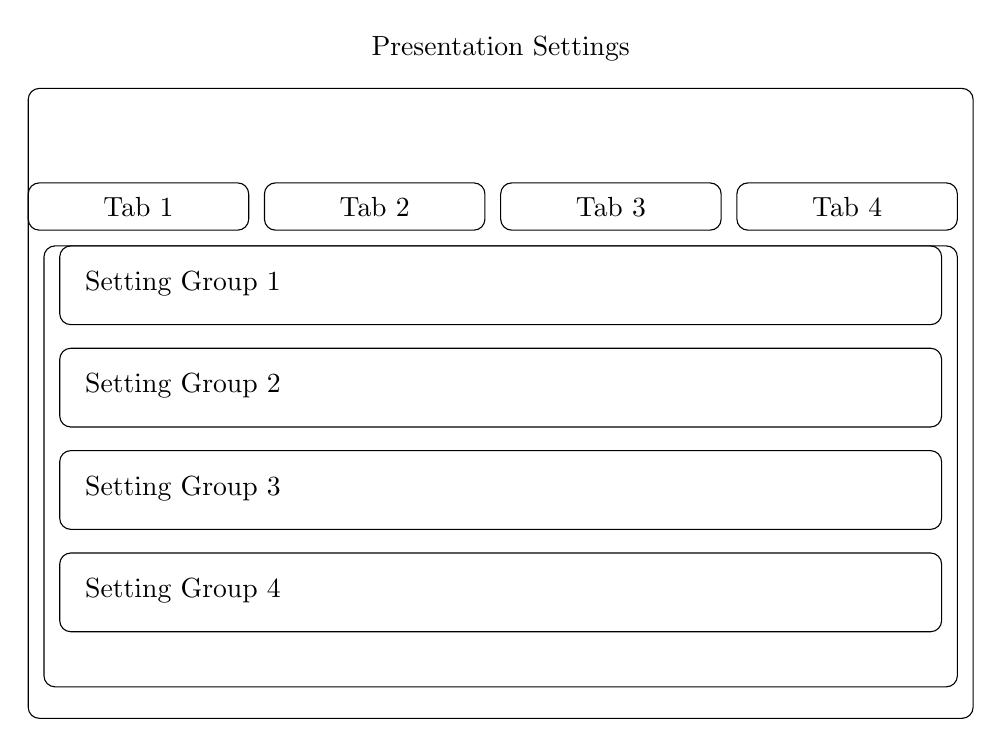
\begin{tikzpicture}
    \begin{scope}
        % Settings dialog
        \draw [rounded corners] (0,0) rectangle (12,-8);
        \node at (6,0.5) {Presentation Settings};

        % Tabs
        \begin{scope}[yshift=-1cm]
            \foreach \x in {0,...,3} {
                \draw [rounded corners] (\x*3,-0.2) rectangle (\x*3+2.8,-0.8);
                \node at (\x*3+1.4,-0.5) {Tab \number\numexpr\x+1\relax};
            }
        \end{scope}

        % Settings panels
        \begin{scope}[yshift=-2cm]
            % General settings
            \draw [rounded corners] (0.2,0) rectangle (11.8,-5.6);

            % Settings groups
            \foreach \y in {0,...,3} {
                \begin{scope}[shift={(0.4,-\y*1.3)}]
                    \draw [rounded corners] (0,0) rectangle (11.2,-1);
                    \node[anchor=north west] at (0.2,-0.2) {Setting Group \number\numexpr\y+1\relax};
                \end{scope}
            }
        \end{scope}
    \end{scope}
\end{tikzpicture}
\caption{Settings Dialog}
\end{figure}

\section{Error Handling and Recovery}

\subsection{Error Management System}
\begin{figure}[H]
\centering
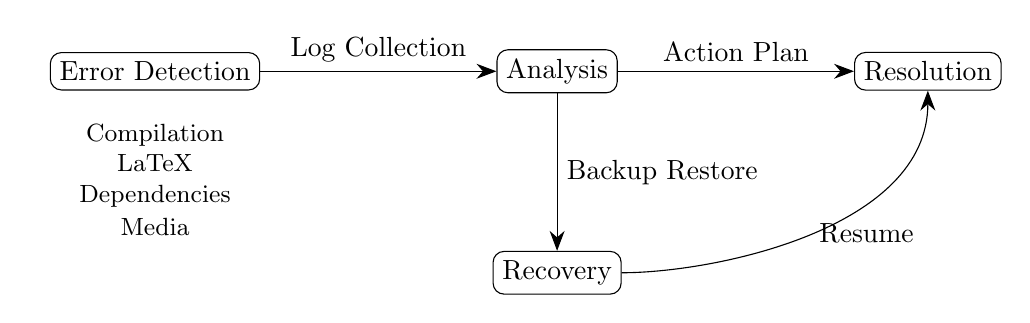
\begin{tikzpicture}
    \begin{scope}
        % Error handling flow diagram
        \node[rectangle, draw, rounded corners, fill=white] (detect) at (0,0) {Error Detection};
        \node[rectangle, draw, rounded corners, fill=white, right=3cm of detect] (analyze) {Analysis};
        \node[rectangle, draw, rounded corners, fill=white, right=3cm of analyze] (resolve) {Resolution};
        \node[rectangle, draw, rounded corners, fill=white, below=2cm of analyze] (recover) {Recovery};

        % Arrows with labels
        \draw[-{Stealth[scale=1.5]}] (detect) -- (analyze)
            node[midway, above] {Log Collection};
        \draw[-{Stealth[scale=1.5]}] (analyze) -- (resolve)
            node[midway, above] {Action Plan};
        \draw[-{Stealth[scale=1.5]}] (analyze) -- (recover)
            node[midway, right] {Backup Restore};
        \draw[-{Stealth[scale=1.5]}] (recover) .. controls +(right:2) and +(down:2) .. (resolve)
            node[midway, right] {Resume};

        % Error types
        \node[below=0.3cm of detect, text width=3cm, align=center]
            {\small Compilation\\LaTeX\\Dependencies\\Media};
    \end{scope}
\end{tikzpicture}
\caption{Error Handling Workflow}
\end{figure}

\subsection{Recovery Features}
\begin{tcolorbox}[title=Automatic Recovery System]
\begin{itemize}
    \item \textbf{Auto-save}: Periodic saving of work
    \item \textbf{Version Control}: Multiple backup points
    \item \textbf{Session Recovery}: State restoration
    \item \textbf{Media Verification}: File integrity checks
\end{itemize}
\end{tcolorbox}

\section{Integration Capabilities}

\subsection{External Tools Integration}
\begin{figure}[H]
\centering
\begin{tikzpicture}
    \begin{scope}
        % Central IDE node
        \node[rectangle, draw, rounded corners, minimum width=4cm, minimum height=2cm,
              fill=white, text=black] (ide) {BSG-IDE};

        % External tool nodes
        \node[rectangle, draw, rounded corners, minimum width=3cm, minimum height=1.5cm,
              fill=white, above=2cm of ide] (latex) {LaTeX Engine};
        \node[rectangle, draw, rounded corners, minimum width=3cm, minimum height=1.5cm,
              fill=white, right=3cm of ide] (pympress) {Pympress};
        \node[rectangle, draw, rounded corners, minimum width=3cm, minimum height=1.5cm,
              fill=white, below=2cm of ide] (youtube) {YouTube-DL};
        \node[rectangle, draw, rounded corners, minimum width=3cm, minimum height=1.5cm,
              fill=white, left=3cm of ide] (overleaf) {Overleaf};

        % Connection arrows with labels
        \draw[-{Stealth[scale=1.5]}] (ide) -- (latex)
            node[midway, right] {Compilation};
        \draw[-{Stealth[scale=1.5]}] (ide) -- (pympress)
            node[midway, above] {Present};
        \draw[-{Stealth[scale=1.5]}] (ide) -- (youtube)
            node[midway, right] {Download};
        \draw[-{Stealth[scale=1.5]}] (ide) -- (overleaf)
            node[midway, above] {Export};
    \end{scope}
\end{tikzpicture}
\caption{External Tool Integration Architecture}
\end{figure}

\section{Performance Optimization}

\subsection{Resource Management}
\begin{figure}[H]
\centering
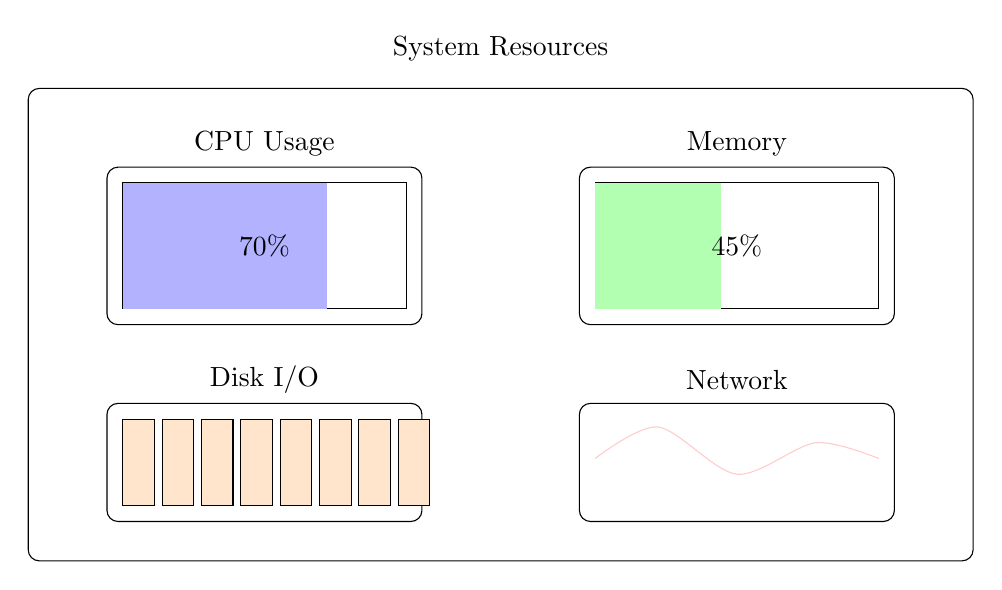
\begin{tikzpicture}
    \begin{scope}
        % Performance monitoring dashboard
        \draw [rounded corners] (0,0) rectangle (12,-6);
        \node at (6,0.5) {System Resources};

        % CPU Usage
        \begin{scope}[shift={(1,-1)}]
            \draw [rounded corners] (0,0) rectangle (4,-2);
            \node at (2,0.3) {CPU Usage};
            \draw (0.2,-0.2) rectangle (3.8,-1.8);
            \fill[blue!30] (0.2,-0.2) rectangle (2.8,-1.8);
            \node at (2,-1) {70\%};
        \end{scope}

        % Memory Usage
        \begin{scope}[shift={(7,-1)}]
            \draw [rounded corners] (0,0) rectangle (4,-2);
            \node at (2,0.3) {Memory};
            \draw (0.2,-0.2) rectangle (3.8,-1.8);
            \fill[green!30] (0.2,-0.2) rectangle (1.8,-1.8);
            \node at (2,-1) {45\%};
        \end{scope}

        % Disk I/O
        \begin{scope}[shift={(1,-4)}]
            \draw [rounded corners] (0,0) rectangle (4,-1.5);
            \node at (2,0.3) {Disk I/O};
            \foreach \x in {0,...,7} {
                \draw[fill=orange!20] (0.2+\x*0.5,-0.2) rectangle (0.6+\x*0.5,-1.3);
            }
        \end{scope}

        % Network
        \begin{scope}[shift={(7,-4)}]
            \draw [rounded corners] (0,0) rectangle (4,-1.5);
            \node at (2,0.3) {Network};
            \draw[red!20] plot[smooth] coordinates {
                (0.2,-0.7) (1,-0.3) (2,-0.9) (3,-0.5) (3.8,-0.7)
            };
        \end{scope}
    \end{scope}
\end{tikzpicture}
\caption{Resource Monitoring Dashboard}
\end{figure}

\section{Collaborative Features}

\subsection{Project Sharing}
\begin{figure}[H]
\centering
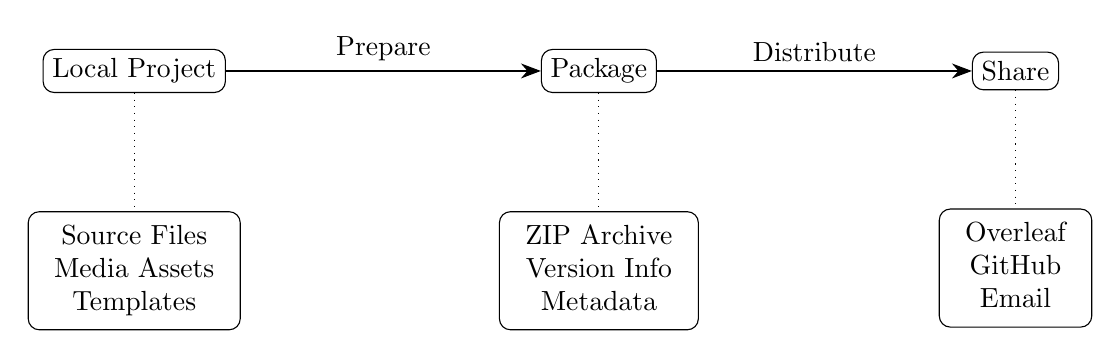
\begin{tikzpicture}
    \begin{scope}
        % Main project workflow
        \node[rectangle, draw, rounded corners, fill=white] (local) at (0,0) {Local Project};
        \node[rectangle, draw, rounded corners, fill=white, right=4cm of local] (package) {Package};
        \node[rectangle, draw, rounded corners, fill=white, right=4cm of package] (share) {Share};

        % Components below each stage
        \node[rectangle, draw, rounded corners, fill=white, below=1.5cm of local] (files) {
            \begin{tabular}{c}
                Source Files\\
                Media Assets\\
                Templates
            \end{tabular}
        };

        \node[rectangle, draw, rounded corners, fill=white, below=1.5cm of package] (bundle) {
            \begin{tabular}{c}
                ZIP Archive\\
                Version Info\\
                Metadata
            \end{tabular}
        };

        \node[rectangle, draw, rounded corners, fill=white, below=1.5cm of share] (platforms) {
            \begin{tabular}{c}
                Overleaf\\
                GitHub\\
                Email
            \end{tabular}
        };

        % Connections
        \draw[-{Stealth[scale=1.5]}] (local) -- (package)
            node[midway, above] {Prepare};
        \draw[-{Stealth[scale=1.5]}] (package) -- (share)
            node[midway, above] {Distribute};

        \draw[dotted] (local) -- (files);
        \draw[dotted] (package) -- (bundle);
        \draw[dotted] (share) -- (platforms);
    \end{scope}
\end{tikzpicture}
\caption{Project Sharing Workflow}
\end{figure}

\section{Best Practices}

\subsection{Project Organization}
\begin{figure}[H]
\centering
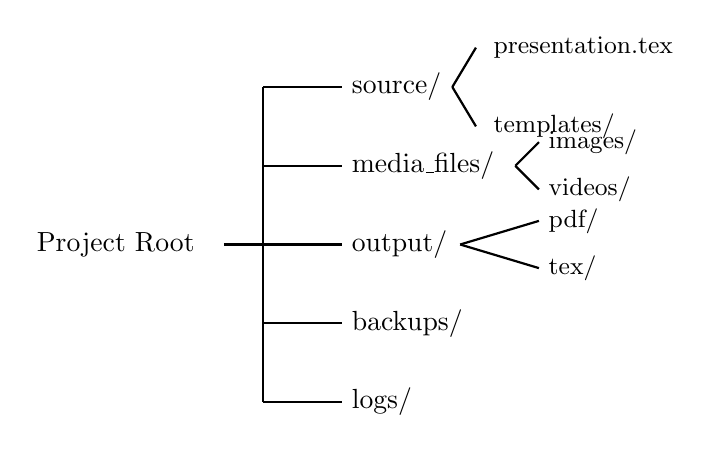
\begin{tikzpicture}
    \begin{scope}
        % Project structure tree
        \node[anchor=west] at (-1,0) {Project Root};
        \draw[thick] (1.5,0) -- (2,0);

        % Main branches
        \foreach \y in {2,1,0,-1,-2} {
            \draw[thick] (2,0) -- (2,\y);
            \draw[thick] (2,\y) -- (3,\y);
        }

        % Labels and sub-branches
        \node[anchor=west] at (3,2) {source/};
        \draw[thick] (4.4,2.) -- (4.7,2.5);
        \draw[thick] (4.4,2) -- (4.7,1.5);
        \node[anchor=west] at (4.8,2.5) {\small presentation.tex};
        \node[anchor=west] at (4.8,1.5) {\small templates/};

        \node[anchor=west] at (3,1) {media\_files/};
        \draw[thick] (5.2,1) -- (5.5,1.3);
        \draw[thick] (5.2,1) -- (5.5,0.7);
        \node[anchor=west] at (5.5,1.3) {\small images/};
        \node[anchor=west] at (5.5,0.7) {\small videos/};

        \node[anchor=west] at (3,0) {output/};
        \draw[thick] (4.5,0) -- (5.5,0.3);
        \draw[thick] (4.5,0) -- (5.5,-0.3);
        \node[anchor=west] at (5.5,0.3) {\small pdf/};
        \node[anchor=west] at (5.5,-0.3) {\small tex/};

        \node[anchor=west] at (3,-1) {backups/};
        \node[anchor=west] at (3,-2) {logs/};
    \end{scope}
\end{tikzpicture}
\caption{Recommended Project Structure}
\end{figure}

\subsection{Performance Guidelines}
\begin{tcolorbox}[title=Optimization Recommendations]
\begin{itemize}
    \item \textbf{Media Files}
        \begin{itemize}
            \item Optimize image sizes before import
            \item Use appropriate formats (JPEG for photos, PNG for diagrams)
            \item Compress video files when possible
        \end{itemize}
    \item \textbf{Project Management}
        \begin{itemize}
            \item Regular cleanup of unused media
            \item Periodic cache clearing
            \item Systematic backup strategy
        \end{itemize}
    \item \textbf{Resource Usage}
        \begin{itemize}
            \item Close unused media previews
            \item Limit concurrent compilations
            \item Monitor memory usage
        \end{itemize}
\end{itemize}
\end{tcolorbox}

\section{Development Roadmap}

\subsection{Future Features}
\begin{figure}[H]
\centering
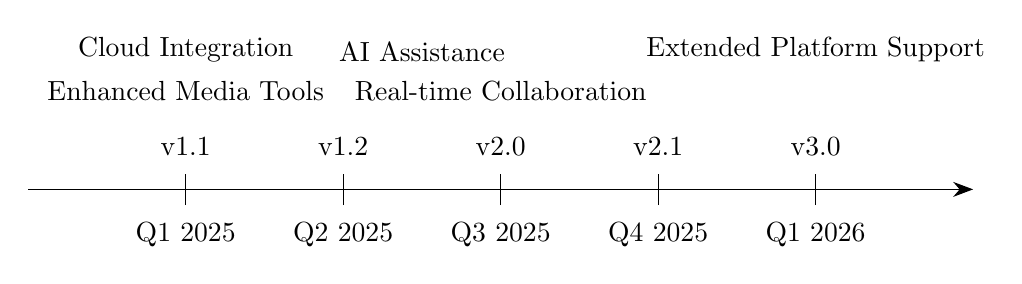
\begin{tikzpicture}
    \begin{scope}
        % Timeline base
        \draw[-{Stealth[scale=1.5]}] (-6,0) -- (6,0);
        \foreach \x in {-4,-2,0,2,4} {
            \draw (\x,-0.2) -- (\x,0.2);
        }

        % Version markers
        \node[above=0.3cm] at (-4,0) {v1.1};
        \node[above=0.3cm] at (-2,0) {v1.2};
        \node[above=0.3cm] at (0,0) {v2.0};
        \node[above=0.3cm] at (2,0) {v2.1};
        \node[above=0.3cm] at (4,0) {v3.0};

        % Feature descriptions
        \node[above=1cm] at (-4,0) {Enhanced Media Tools};
        \node[above=1cm] at (-4,0.5) {Cloud Integration};
        \node[above=1cm] at (0,0) {Real-time Collaboration};
        \node[above=1cm] at (-1,0.5) {AI Assistance};
        \node[above=1cm] at (4,0.5) {Extended Platform Support};

        % Time indicators
        \node[below=0.3cm] at (-4,0) {Q1 2025};
        \node[below=0.3cm] at (-2,0) {Q2 2025};
        \node[below=0.3cm] at (0,0) {Q3 2025};
        \node[below=0.3cm] at (2,0) {Q4 2025};
        \node[below=0.3cm] at (4,0) {Q1 2026};
    \end{scope}
\end{tikzpicture}
\caption{Development Timeline}
\end{figure}

\section{Appendices}

\subsection{LaTeX Package Requirements}
\begin{tcolorbox}[title=Required LaTeX Packages]
\begin{lstlisting}[language=TeX]
% Core packages
\usepackage{beamer}
\usepackage{graphicx}
\usepackage{multimedia}
\usepackage{hyperref}

% Enhanced functionality
\usepackage{tikz}
\usepackage{pgfplots}
\usepackage{animate}

% Customization
\usepackage{tcolorbox}
\usepackage{geometry}
\usepackage{fancyhdr}
\usepackage{xcolor}

% Font and encoding
\usepackage[T1]{fontenc}
\usepackage{lmodern}
\usepackage[utf8]{inputenc}
\end{lstlisting}
\end{tcolorbox}

\subsection{Python Dependencies}
\begin{tcolorbox}[title=Required Python Packages]
\begin{lstlisting}[language=Python]
# GUI Framework
customtkinter==5.2.2
tkinter
Pillow

# Media Processing
opencv-python
yt-dlp
screeninfo

# PDF Generation
PyMuPDF==1.23.7

# Utilities
requests
numpy
\end{lstlisting}
\end{tcolorbox}

\subsection{File Format Specifications}

\begin{figure}[H]
\centering
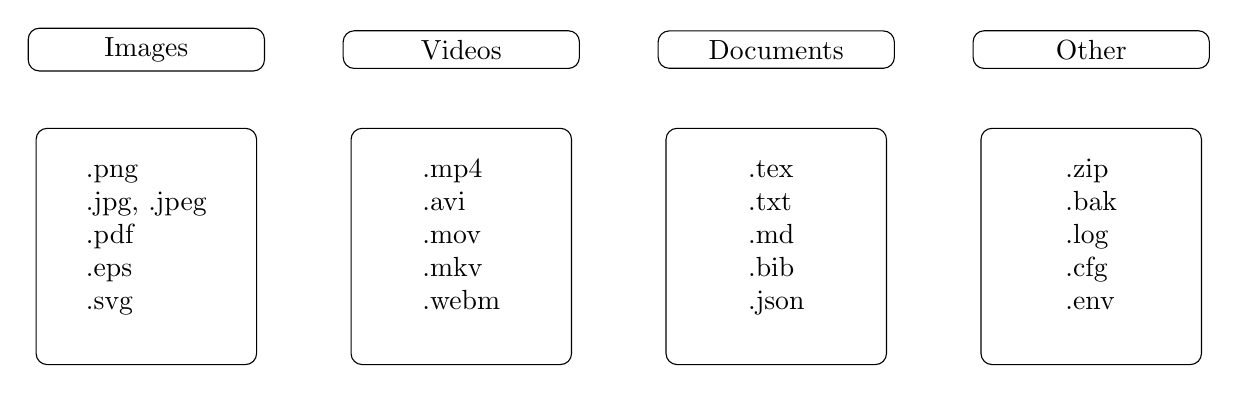
\begin{tikzpicture}
    \begin{scope}
        % Main categories with file types
        \node[rectangle, draw, rounded corners, minimum width=3cm, fill=white] (images) at (0,0) {Images};
        \node[rectangle, draw, rounded corners, minimum width=3cm, fill=white] (videos) at (4,0) {Videos};
        \node[rectangle, draw, rounded corners, minimum width=3cm, fill=white] (docs) at (8,0) {Documents};
        \node[rectangle, draw, rounded corners, minimum width=3cm, fill=white] (other) at (12,0) {Other};

        % File types for each category
        \foreach \i in {0,...,3} {
            \draw[rounded corners] (\i*4-1.4,-1) rectangle (\i*4+1.4,-4);
        }

        % Image formats
        \node[anchor=north] at (0,-1.2) {
            \begin{tabular}{l}
                .png\\
                .jpg, .jpeg\\
                .pdf\\
                .eps\\
                .svg
            \end{tabular}
        };

        % Video formats
        \node[anchor=north] at (4,-1.2) {
            \begin{tabular}{l}
                .mp4\\
                .avi\\
                .mov\\
                .mkv\\
                .webm
            \end{tabular}
        };

        % Document formats
        \node[anchor=north] at (8,-1.2) {
            \begin{tabular}{l}
                .tex\\
                .txt\\
                .md\\
                .bib\\
                .json
            \end{tabular}
        };

        % Other formats
        \node[anchor=north] at (12,-1.2) {
            \begin{tabular}{l}
                .zip\\
                .bak\\
                .log\\
                .cfg\\
                .env
            \end{tabular}
        };
    \end{scope}
\end{tikzpicture}
\caption{Supported File Formats}
\end{figure}

\subsection{Configuration Reference}

\begin{tcolorbox}[title=Sample Configuration File]
\begin{lstlisting}[language=Python]
# config.json
{
    "editor": {
        "theme": "dark",
        "font_size": 12,
        "auto_save": true,
        "save_interval": 300,
        "syntax_highlighting": true
    },
    "compilation": {
        "auto_compile": true,
        "compiler": "pdflatex",
        "bibtex_enabled": true,
        "clean_auxiliary": true
    },
    "media": {
        "thumbnail_size": [200, 200],
        "cache_enabled": true,
        "max_cache_size": 1024,
        "supported_formats": ["png", "jpg", "mp4", "pdf"]
    },
    "paths": {
        "output_dir": "./output",
        "media_dir": "./media_files",
        "backup_dir": "./backups",
        "temp_dir": "/tmp/bsg-ide"
    }
}
\end{lstlisting}
\end{tcolorbox}

\subsection{Troubleshooting Guide}

\begin{tcolorbox}[title=Common Issues and Solutions]
\begin{itemize}
    \item \textbf{Installation Issues}
        \begin{itemize}
            \item Run with --fix flag
            \item Check system requirements
            \item Verify Python version
            \item Check LaTeX installation
        \end{itemize}
    \item \textbf{Compilation Errors}
        \begin{itemize}
            \item Verify LaTeX syntax
            \item Check media file paths
            \item Ensure all packages are installed
            \item Review log files
        \end{itemize}
    \item \textbf{Media Problems}
        \begin{itemize}
            \item Verify file permissions
            \item Check file formats
            \item Ensure media directory exists
            \item Review conversion settings
        \end{itemize}
    \item \textbf{Performance Issues}
        \begin{itemize}
            \item Clear cache
            \item Optimize media files
            \item Close unused previews
            \item Monitor resource usage
        \end{itemize}
\end{itemize}
\end{tcolorbox}

\subsection{Command Line Interface}

\begin{tcolorbox}[title=CLI Commands]
\begin{lstlisting}[language=bash]
# Basic usage
bsg-ide                    # Launch GUI
bsg-ide --fix             # Repair installation
bsg-ide --help            # Show help

# Advanced options
bsg-ide --no-gui          # Terminal mode
bsg-ide --compile file.tex # Direct compilation
bsg-ide --clean           # Clean temporary files
bsg-ide --version         # Show version info
\end{lstlisting}
\end{tcolorbox}

\section{Index}

\begin{multicols}{2}
\begin{itemize}
    \item Installation, 2
    \item Media Management, 5
    \item Notes System, 7
    \item Keyboard Shortcuts, 9
    \item Project Organization, 11
    \item Error Handling, 13
    \item External Tools, 15
    \item Performance, 17
    \item Collaboration, 19
    \item Development Roadmap, 21
    \item Configuration, 23
    \item Troubleshooting, 25
\end{itemize}
\end{multicols}

\end{document}
